\documentclass[margin=0mm,tikz]{standalone}

\usepackage{tikz}
\usepackage{xcolor}

\usetikzlibrary{positioning}
\usetikzlibrary{fit}
\usetikzlibrary{calc}
\usetikzlibrary{arrows.meta}
\usetikzlibrary{quotes}
\usetikzlibrary{backgrounds}

\pgfdeclarelayer{background}
\pgfsetlayers{background,main}

% -----------------------
% colors
% -----------------------
\definecolor{facecolor}{RGB}{24, 127, 206}

% Set background color
%\pagecolor{white}


\tikzstyle{cface} = [
    thick, 
    draw=facecolor!50!gray,
    top color = facecolor!20!white,
    bottom color = facecolor!30!white,
    minimum size=1.5cm,
]
\tikzstyle{nface} = [
	thick, 
	draw=facecolor!50!gray,
	top color = facecolor!20!white,
	bottom color = facecolor!30!white,
	minimum size=1.5cm,
	opacity=0.5
]
\tikzstyle{diag} = [
	dotted,
	opacity=0.5
]


\begin{document}
	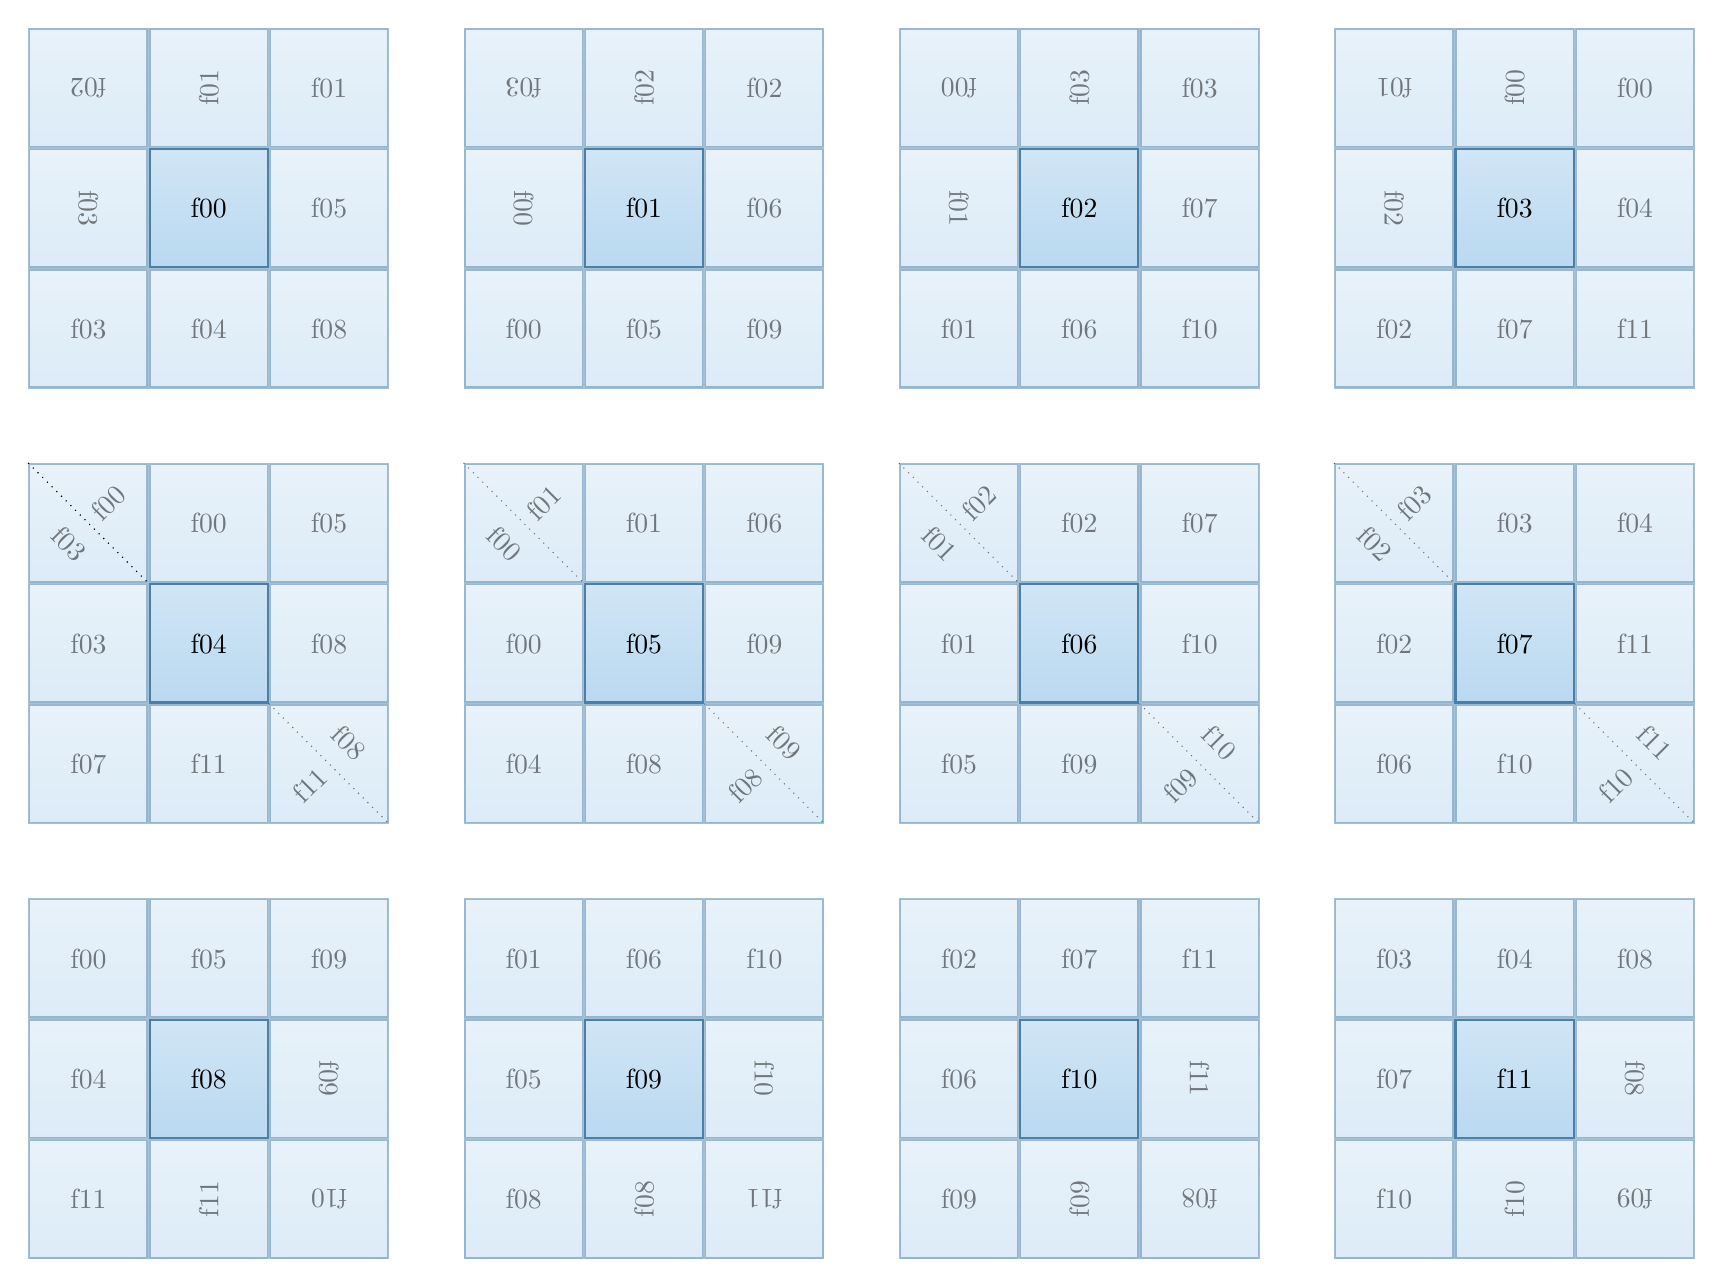
\begin{tikzpicture}[node distance=0cm and 0cm]
	
	%
	% North faces
	\node[cface] (f00) {f00};
	\node[nface, above=of f00] {\rotatebox{90}{f01}};
	\node[nface, above left=of f00] {\rotatebox{180}{f02}};
	\node[nface, left=of f00] {\rotatebox{270}{f03}};
	\node[nface, below left=of f00] {f03};
	\node[nface, below=of f00] {f04};
	\node[nface, below right=of f00] {f08};
	\node[nface, right=of f00] {f05};
	\node[nface, above right=of f00] {f01};
	
	\node[cface, right=of f00, xshift=4cm] (f01) {f01};
	\node[nface, above=of f01] {\rotatebox{90}{f02}};
	\node[nface, above left=of f01] {\rotatebox{180}{f03}};
	\node[nface, left=of f01] {\rotatebox{270}{f00}};
	\node[nface, below left=of f01] {f00};
	\node[nface, below=of f01] {f05};
	\node[nface, below right=of f01] {f09};
	\node[nface, right=of f01] {f06};
	\node[nface, above right=of f01] {f02};
	
	\node[cface, right=of f01, xshift=4cm] (f02) {f02};
	\node[nface, above=of f02] {\rotatebox{90}{f03}};
	\node[nface, above left=of f02] {\rotatebox{180}{f00}};
	\node[nface, left=of f02] {\rotatebox{270}{f01}};
	\node[nface, below left=of f02] {f01};
	\node[nface, below=of f02] {f06};
	\node[nface, below right=of f02] {f10};
	\node[nface, right=of f02] {f07};
	\node[nface, above right=of f02] {f03};
	
	\node[cface, right=of f02, xshift=4cm] (f03) {f03};
	\node[nface, above=of f03] {\rotatebox{90}{f00}};
	\node[nface, above left=of f03] {\rotatebox{180}{f01}};
	\node[nface, left=of f03] {\rotatebox{270}{f02}};
	\node[nface, below left=of f03] {f02};
	\node[nface, below=of f03] {f07};
	\node[nface, below right=of f03] {f11};
	\node[nface, right=of f03] {f04};
	\node[nface, above right=of f03] {f00};
	
	%
	% Equator faces
	\node[cface, below=of f00, yshift=-4cm] (f04) {f04};
	\node[nface, above=of f04] {f00};
	\node[nface, above left=of f04] (f04nw) {\rotatebox[origin=c,x=-0.5cm]{-45}{f03}\rotatebox[origin=c]{45}{f00}};
	\draw[dotted] (f04nw.north west)--(f04nw.south east);
	\node[nface, left=of f04] {f03};
	\node[nface, below left=of f04] {f07};
	\node[nface, below=of f04] {f11};
	\node[nface, below right=of f04] (f04se) {\rotatebox[origin=c, x=1cm]{45}{f11}\rotatebox[origin=c]{-45}{f08}};
	\draw[diag] (f04se.north west)--(f04se.south east);
	\node[nface, right=of f04] {f08};
	\node[nface, above right=of f04] {f05};
	
	\node[cface, below=of f01, yshift=-4cm] (f05) {f05};
	\node[nface, above=of f05] {f01};
	\node[nface, above left=of f05] (f05nw) {\rotatebox[origin=c,x=-0.5cm]{-45}{f00}\rotatebox[origin=c]{45}{f01}};
	\draw[diag] (f05nw.north west)--(f05nw.south east);
	\node[nface, left=of f05] {f00};
	\node[nface, below left=of f05] {f04};
	\node[nface, below=of f05] {f08};
	\node[nface, below right=of f05] (f05se) {\rotatebox[origin=c, x=1cm]{45}{f08}\rotatebox[origin=c]{-45}{f09}};
	\draw[diag] (f05se.north west)--(f05se.south east);
	\node[nface, right=of f05] {f09};
	\node[nface, above right=of f05] {f06};
	
	\node[cface, below=of f02, yshift=-4cm] (f06) {f06};
	\node[nface, above=of f06] {f02};
	\node[nface, above left=of f06] (f06nw) {\rotatebox[origin=c,x=-0.5cm]{-45}{f01}\rotatebox[origin=c]{45}{f02}};
	\draw[diag] (f06nw.north west)--(f06nw.south east);
	\node[nface, left=of f06] {f01};
	\node[nface, below left=of f06] {f05};
	\node[nface, below=of f06] {f09};
	\node[nface, below right=of f06] (f06se) {\rotatebox[origin=c, x=1cm]{45}{f09}\rotatebox[origin=c]{-45}{f10}};
	\draw[diag] (f06se.north west)--(f06se.south east);
	\node[nface, right=of f06] {f10};
	\node[nface, above right=of f06] {f07};
	
	\node[cface, below=of f03, yshift=-4cm] (f07) {f07};
	\node[nface, above=of f07] {f03};
	\node[nface, above left=of f07] (f07nw) {\rotatebox[origin=c,x=-0.5cm]{-45}{f02}\rotatebox[origin=c]{45}{f03}};
	\draw[diag] (f07nw.north west)--(f07nw.south east);
	\node[nface, left=of f07] {f02};
	\node[nface, below left=of f07] {f06};
	\node[nface, below=of f07] {f10};
	\node[nface, below right=of f07] (f07se) {\rotatebox[origin=c, x=1cm]{45}{f10}\rotatebox[origin=c]{-45}{f11}};
	\draw[diag] (f07se.north west)--(f07se.south east);
	\node[nface, right=of f07] {f11};
	\node[nface, above right=of f07] {f04};
	
	%
	% South faces
	\node[cface, below=of f04, yshift=-4cm] (f08) {f08};
	\node[nface, above=of f08] {f05};
	\node[nface, above left=of f08] {f00};
	\node[nface, left=of f08] {f04};
	\node[nface, below left=of f08] {f11};
	\node[nface, below=of f08] {\rotatebox{90}{f11}};
	\node[nface, below right=of f08] {\rotatebox{180}{f10}};
	\node[nface, right=of f08] {\rotatebox{270}{f09}};
	\node[nface, above right=of f08] {f09};
	
	\node[cface, below=of f05, yshift=-4cm] (f09) {f09};
	\node[nface, above=of f09] {f06};
	\node[nface, above left=of f09] {f01};
	\node[nface, left=of f09] {f05};
	\node[nface, below left=of f09] {f08};
	\node[nface, below=of f09] {\rotatebox{90}{f08}};
	\node[nface, below right=of f09] {\rotatebox{180}{f11}};
	\node[nface, right=of f09] {\rotatebox{270}{f10}};
	\node[nface, above right=of f09] {f10};
	
	\node[cface, below=of f06, yshift=-4cm] (f10) {f10};
	\node[nface, above=of f10] {f07};
	\node[nface, above left=of f10] {f02};
	\node[nface, left=of f10] {f06};
	\node[nface, below left=of f10] {f09};
	\node[nface, below=of f10] {\rotatebox{90}{f09}};
	\node[nface, below right=of f10] {\rotatebox{180}{f08}};
	\node[nface, right=of f10] {\rotatebox{270}{f11}};
	\node[nface, above right=of f10] {f11};

	\node[cface, below=of f07, yshift=-4cm] (f11) {f11};
	\node[nface, above=of f11] {f04};
	\node[nface, above left=of f11] {f03};
	\node[nface, left=of f11] {f07};
	\node[nface, below left=of f11] {f10};
	\node[nface, below=of f11] {\rotatebox{90}{f10}};
	\node[nface, below right=of f11] {\rotatebox{180}{f09}};
	\node[nface, right=of f11] {\rotatebox{270}{f08}};
	\node[nface, above right=of f11] {f08};
	
		
	\end{tikzpicture}
\end{document}